\documentclass{tktltiki}
\usepackage[pdftex]{graphicx}
\usepackage{subfigure}
\usepackage{url}
\usepackage{amsmath}
\usepackage{lmodern}
\begin{document}
%\doublespacing
%\singlespacing
\onehalfspacing

\title{Mutaatiotestaus -- working title}
\author{Tony Kovanen}
\date{\today}

\maketitle

\numberofpagesinformation{\numberofpages\ sivua + \numberofappendixpages\ liitesivua}
\classification{\protect{\ \\
A.1 [Introductory and Survey],\\
I.7.m [Document and text processing]}}

\keywords{Ohjelmistojen testaus, mutatointi, testidatan generointi}

\mytableofcontents

\section{Johdanto}
Ohjelmistoja tuotettaessa on tärkeää validoida ohjelmiston eri komponenttien toimivuus, niiden yhteensopivuus, sekä järjestelmän toimivuus kokonaisuudessaan. Testauksen rooli ohjelmistotuotantoprosessissa vie potentiaalisesti paljon resursseja verrattuna muuhun prosessissa vaadittuun työmäärään, mutta se myös torjuu tehokkaasti viallista koodia~\cite{}. Vaikka testaus ei anna täysin objektiivista totuutta siitä toimiiko ohjelmisto kuten on odotettu, se kuitenkin kasvattaa sen luotettavuutta. Kattavien testien läsnäollessa voidaan myös huoletta lisätä uutta toiminnallisuutta, muokata vanhaa toiminnallisuutta, ja refaktoroida ohjelmakoodia, sillä epäonnistuvat testit indikoivat sitä, että jotain on rikottu näitä muutoksia tehtäessä, eikä koodin muokkaaminen näinollen tuo prosessiin yhtä paljon epävarmuutta ohjelmiston toimivuuden suhteen.

\subsection{Testauksen tasot}
Yksikkötesteillä huolehditaan siitä, että yksittäiset komponentit ohjelmistossa toimivat oikein. Näillä voidaan varmistaa olio-ohjelmointikielissä yksittäisten luokkien ja niiden metodien toimivuus. Vastaavia testejä voidaan kirjoittaa myös esimerkiksi funktionaalisiin ohjelmointikieliin, joissa yksikkötestit testaavat yksittäisten funktioiden toiminnallisuutta. Kattavien yksikkötestien läsnäollessa refaktorointi on helpompaa, sillä jokaisen muutoksen jälkeen voidaan ajaa yksikkötestit, ja saada välitöntä palautetta siitä toimiiko muutettu komponentti vieläki olennaisesti samalla tavalla.

Integraatiotestit testaavat komponenttien toimivuutta kokonaisuutena. Integraatiotestejä voidaan kirjoittaa useilla yksikkötesteihin ominaisilla testikehyksillä, mutta niitä varten on myös suunniteltu monia omia ohjelmakehityksiä. Integraatioestit on usein toteutettu ihmismäistä käyttäytymistä imitoiviksi, esimerkiksi selainympäristössä suoritettaville ohjelmistoille on kehitetty erilaisia kirjastoja, joilla voidaan avata ohjelmisto selaimessa, ja navigoida sivulla aivan kuten ihminen. Toimivuus voidaan sitten validoida odotettujen näkymien ja HTTP statuskoodien perusteella.

\subsection{Testikattavuus}
Niin yksikkö- kuin integraatiotestien yhteydessä puhutaan usein testikattavuudesta. Testikattavuus on mitta siitä, miten hyvin käytettävät testit kattavat komponenttien tarjoaman toiminnallisuuden, tai koko järjestelmälle määritellyn toiminnallisuuden. Kattavuuden mittana tunnetuimmat ja yleisimmät ovat rivikattavuus, ja haarakattavuus.

Rivikattavuus mittaa testattavasta komponetista testien käsittelemän ohjelmakoodin rivien määrän. Jos jonkin komponentin yksikkötestit suoritettaessa suorittavat jokaisen rivin komponentin ohjelmakoodista, on rivikattauus 100\%, ja pidetään komponentin testejä tämän metriikan nojalla kattavana.

Haarakattavuus mittaa eri kontrollirakenteista syntyvien haarojen kattavuuden, eli se kertoo prosentuaalisesti sen määrän eri kontrollihaaroista, minkä ohjelmakoodin testit ovat suorittaneet testattavasta komponentista. Jos jokainen haara käsitellään testeissä, ovat testit haarakattavuuden nojalla kattavat. Useimmiten testikattavuuden mittana käytetään näiden kahden mitan unionia, sillä molemmat ovat yksinään hyvin puutteellisia.

Rivi- ja haarakattavuuden lisäksi on olemassa muita mittoja testikattavuuden mittaamiseen, joista yksi on mutaatiokattavuus. Mutaatiokattavuudella pyritään semanttisempaan analyysin testien kattavuudesta. Mutaatioestauksen tavoite on saada selville kuinka kattavasti määritellyt testit löytävät ohjelmakoodiin indusoitavia pieniä muutoksia. Tässä tutkielmassa esitellään mutaatiotestaus, sen menetelmät, sovellukset ja heikkoudet.

\section{Mutaatiotestaus}
Mutaatiotestaus on menetelmä jolla voidaan mitata jonkin testijoukon virheenhavaitsemiskykyä. Mutaatioestaus tapahtuu ohjelmalle suoritettavalla testaussyklillä. Ensin ohjelman testit ajetaan alkuperäiselle lähdekoodille. Jos jokin testi epäonnistuu, pitää se korjata ennen jatkamista.

Seuraavaksi ohjelmakoodista tehdään useita kopioita, joissa joku yksityiskohta, tai joitain yksityiskohtia on muutettu niinsanotuilla mutaatioilla. Näitä kopioita kutsutaan mutanteiksi, jotka esittävät mahdollisia virheellisiä variantteja alkuperäisestä ohjelmasta. Testit jotka on annettu mutaatiosyklin parametreina ajetaan jokaiselle mutantille. Jos jokin testi epäonnistuu mutantin kohdalla, tämä mutantti leimataan tapetuksi, sillä tämä testi tunnisti koodin tehdyn muutoksen. Jos taas mikään testi ei epäonnistu, mutantti leimataan selviytyjäksi, sillä mikään testi ei tunnistanut muutosta. Selvitytyneet mutantit kielivät usein puutteesta testeissä. Jokaisesta mutantista otetaan usein talteen mutaatiokohta, sekä mutaatio. Näin selviytynyeitä mutantteja voidaan tarkastella, ja testejä parannella selviytyneitä mutantteja apuna käyttäen. Ne antavat usein vihjeitä siitä mikä testeissä on puutteellista. Mutaatioestauksen mittana käytetään mutaatiokattavuutta, joka lasketaan yksinkertaisesti kaavalla $\frac{k}{t}$, missä $k$ tarkoittaa tapettuja mutantteja, ja $t$ tarkoittaa mutanttien kokonaismäärää.

Mutaatiosykliin ollaan ehdoteltu parannuksia. Lupaavia lisäyksiä tutkitaan jatkuvasti, ja tulevaisuuden varalle ollaan ehdotettu seuraavaa pidennystä sykliin: kun selviytyvät mutantit ollaan löydetty generoidaan niiden perusteelta testejä automaattisesti. Toistetaan sitten sykliä alusta lähtien niin kauan kunnes yksikään mutantti ei jää henkiin. Tähän sykliin pääseminen ei ole kuitenkaan vielä mahdollista. Mutaatiotestaukseen liittyvät ongelmat käsitellään myöhemmissä kappaleissa.

\section{Mutaatiot}
Mutaatiotestaus perustuu siihen, että ohjelmakoodiin indusoidaan mutaatoita, joita ohjelmalle määriteltyjen testien tulisi huomata. Mutaatio tarkoittaa perinnöllisyystieteessä muutosta geeniin jossa yksi geenin kemiallinen komponentti, nulkeotidi, on vaihtunut joksikin toiseksi, on deletoitu sekvenssistä, tai on insertoitu sekvenssiin. Ohjelmakoodiin indusoitavat mutaatiot on toteutettu samalla idealla: koodista voidaan esim. poistaa yksittäisiä rivejä, muuntaa operaattoreita tai metodikutsuja toisiksi, tai lisätä ylimääräistä koodia. Mahdollisia mutaatoita on siis erittäin suuri määrä, ja laskennallisista syistä niistä usein halutaan käyttää vain osajoukkoa. Tyypilliset mutaatiot tuodaan esille myöhemmin tässä kappaleessa. Ensin kuitenkin esitellään mutaatioiden konsepti tarkemmin, sekä miten ne ilmenevät eri ohjemointikielissä.

\begin{figure}[here]
\caption{Äärellinen automaatti $O$ joka hyväksyy minkä tahansa lukuun $1$ päättyvän aakkoston $\Sigma = \{0,1\}$ sekvenssin.}
\label{fig:nfa}
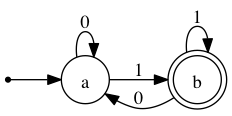
\includegraphics{automaatit/nfa.png}
\end{figure}

\begin{figure}[here]
\caption{Ensimmäisen asteen mutantti $m1$ automaatista $O$, jossa siirtymä tilasta $b$ tilaan $a$ on lisätty aakkosella $1$}
\label{fig:m1}
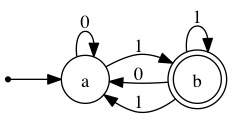
\includegraphics{automaatit/m1.png}
\end{figure}

\begin{figure}[here]
\caption{Ensimmäisen asteen mutantti $m2$ automaatista $O$, jossa siirtymä tilasta $a$ tilaan $b$ korvattu tyhjällä siirtymällä}
\label{fig:m2}
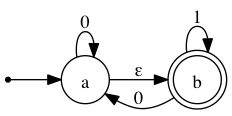
\includegraphics{automaatit/m2.png}
\end{figure}

\subsection{Mutaatiot äärellisillä automaateilla}
Mutaatiot on helppo esittää äärellisillä automaateilla. Olkoon $\Sigma=\{0,1\}$ aakkosto. Voimme nyt määritellä tälle aakkostolle useita eri äärellisiä automaatteja, jotka hyväksyvät vain jotkin tietyt merkkijonot joka koostuvat aakkosista $\sigma \in \Sigma$. Eräs tällainen automaatti löytyy kuvasta~\ref{fig:nfa}, jonka aloitustila on tila $a$ ja hyväksyvä tila on $b$. Kyseinen automaatti hyväksyy minkä tahansa tilasiirtymäsekvenssin, joka loppuu aakkoseen $\sigma = 1$. Määritellään nyt myös joukko mutaatioita $M$. Jokainen mutaatio $m\in M$ on kuvaus, joka korvaa jonkin olemassaolevan tilasiirtymän toisella, poistaa tilasiirtymän, tai lisää tilasiirtymän. Näitä funktioita kutsutaan mutaatio-operaattoreiksi. Jokainen mutaatio $m$ on siis kuvaus aakkoston $\Sigma$ äärellisten automaattien joukolta itselleen, jossa tämä mutaatio tekee jonkn muutoksen, tai joitakin muutoksia annettuun äärelliseen automaattiin. Tarkastellaan joitain kuvan~\ref{fig:nfa} epädeterministisen äärellisen automaatin ensimmäisen asteen mutantteja eli mutaatioita, jotka sisältävät vain yhden edellämainitun muutoksen alkuperäiseen automaattiin. 

Kuva~\ref{fig:m1} ja ~\ref{fig:m2} sisältävät eräät ensimmäisen asteen mutantit alkuperäisestä automaatista. Kuvan~\ref{fig:m1} mutantti on eroaa sillä, että toinen yhteys tilasta $b$ tilaan $a$ on lisätty. Mutantti kuvassa~\ref{fig:m2} eroaa alkuperäisestä automaatista siten, että yhteys tilasta $a$ tilaan $b$ on vaihdettu tyhjäksi siirtymäksi. Kun tarkastelemme millaisia tilasiirtymäsekvenssejä nämä mutanttiautomaatit hyväksyvät, huomaamme että kuvan~\ref{fig:m2} automaatti ei ole funktionaalisesti sama kuin alkuperäinen automaatti kuvassa~\ref{fig:nfa}. Kuvan~\ref{fig:m2} mutantti hyväksyy minkä tahansa tilasiirtymäsekvenssin annetulla aakkostolla $\Sigma$, sillä tyhjä tilasiirtymä vie hyväksyvään tilaan $b$. Tilasta $b$ voidaan siirtyä nollasiirtymällä tilaan $a$, tai ykkössiirtymällä itseensä. Mikäli siirrytään tilaan $a$, voidaan pysyä tässä tilassa nollasiirtymällä, tai siirtyä hyväksyvään tilaan tyhjällä siirtymällä. Huomataan siis, että $L(O) \neq L(m2)$, eli alkuperäisen automaatin määrittelemä kieli $L(0)$ ei ole sama kuin kuvan~\ref{fig:m2} määrittelä kieli $L(m2)$.

Kun tarkastellaan kuvan~\ref{fig:m1} mutanttia $m1$, huomataan, että se hyväksyy täsmälleen samat tilasiirtymäsekvenssit kuin alkuperäinen automaatti $O$, eli $L(O) = L(m1)$, sillä $m1$ hyväksyy ne sekvenssit, jotka jokin mahdollinen tilasiirtymäsarja hyväksyy. Mutantissa $m1$ on kaikki samat tilasiirtymät kuin automaatissa $O$, joten se hyväkyy vähintään kaikki samat sekvenssit. Tämä automaatti ei myöskään hyväksy mitään muita sekvenssejä, sillä lisätty tilasiirtymä ei tuo mitään uusia mahdollisuuksia siirtyä hyväksyvään tilaan $b$, vaan ainoastaan pois siitä. Päästäkseen takaisin tilaan $b$ on taas käytettävä ykkössiirtymää. Tilannetta, jolloin $L(0) = L(m1)$ kutsutaan ekvivalenssiksi. Vaikka $O \neq m1$, ovat ne funktionaalisesti samat, eli niiden kielet ovat samat. 
 
\subsection{Mutaatiot ohjelmointikielissä}
Mutaatiot on helppo laajentaa äärellisiltä automaateilta ohjelmointikielille. Olkoon $O$ jokin alkuperäinen, jollain ohjelmointikielellä toteutettu ohjelma. Nyt $M$ on joukko mutantteja. Nyt jokainen $m\in M$ on sama ohjelma, johon on tehty jokin tai joitakin syntaktisia muutoksia. Mutaatoiden luonto riippuu usein käyteystä alustasta. On selvää, että täysin samat mutaatiot eivät käy sekä imperatiivisiin olio-ohjelmointikieliin, kun puhtaasti funktionaalisiin ohjelmointikieliin. Esimeriksi Javan mutaatiotestauskehysten mutaatiot eivät ole kovinkaan sopivia Clojuren mutaatiotestauskehyksen mutaatioiksi. 

Mutantit tuotetaan ohjelmointikieliin ns. mutaatio-operaattoreilla. Mutaatio-operaattori on funktio joka tuottaa mutaation annettuun ohjelmaan $O$. Idea mutaatiolle on täysin sama kuin äärellisille automaateille. Voidaan korvata, lisätä tai poistaa elementtejä ohjelmakoodista. Käytettävät mutaatio-operaattorit ovat imperatiivisissa ohjelmointikielissä pääosin samat. Agrawal ja kumppanit listaavat 76 C-kielen mutaatio-operaattoria. Nämä mutaatio-operaattorit pätevät pääosin siis kaikkiin C-pohjaisiin ohjelmointikieliin, kuten Javaan ja PHP:hen, sekä karkeasti kaikkiin muihin imperatiivisiin ohjelmointikieliin. Ne ovat jaettu seuraaviin ryhmiin: lausemutaatio, operaattorimutaatio, muuttujamutaatio, vakiomutaatio. Lausemutaatioihin luetaan mm. breakin muuttaminen continue lauseeseen, sekä aaltosulkeiden paikanmuuttaminen ja goto lauseen kohteen muuttaminen. Operaattorimutaatioita ovat esimerkiksi aritmeettisten ja loogisten operaattoreiden muuttamiset toisiksi. Muuttujien mutatointia ovat mm. viitteiden vaihtaminen toiseksi. Vakioiden mutatointi viittaa vakioiden arvojen päittäin vaihtamiseen, tai yksittäisen vakion arvon manipulointiin. Jokaisesta näistä mutaatiotyypistä on useita variaatioita, ja joistakin lähteistä vastaavanlaisia mutaatio-operaattoreita löytyy jopa enemmän. Proteumissa, Delamaron ja Maldonadon esittelemässä mutaatiotestikehyksessä C-kielelle, on jopa 108 mutaatio-operaattoria~\cite{}. 

\subsection{Mutaatiot eri ohjemointiparadigmoissa}
Ohjelmointikielen paradigma voi tuoda mukanaan muutoksia. Esimerkiksi Javassa, sekä muissa olio-ohjelmointikielissä voidaan kokea tarve sen olio-ohjelmointiominaisuuksiin spesifeille operaattoreille. Kim ja kumppanit esittelevät useita olio-ohjelmontispesifejä mutaatio-operaattoreita, kuten metodien parametrien järjestyksen vaihtaminen, ylikuormituksen poistaminen, metodien ylikirjoitus perinnässä ja monia muita~\cite{}. Näiden uusien mutaatio-operaattoreiden lisäksi luokkien sisäistä ohjelmakoodia tulee mutatoida. Mutantteja ei luoda vain pääohjelmasta, vaan jokainen ohjelman yksittäinen komponentti mutatoidaan käytössä olevia mutaatio-operaattoreita käyttäen. Mutaatio-operaattoreita voidaan lisätä olio-ohjelmointikieliinkin suuria määriä. Voidaan kuitenkin miettiä ovatko kaikki operaatorit tarpeellisia. Tarpeellista määrä mutaatio-operaattoreita sanotaan riittäväksi joukoksi.

Olio-ohjelmointispesifeistä mutaatio-operaattoreista jo huomattiin, etä paradiman vaihtuessa myös mutaatiotaktiikkaa tulee muuttaa. Tämä ei päde ainoastaan olio-ohjelmointiparadigmaan. Mutatoitaessa jotain puhtaasti funktionaalista ohjelmointikieltä, kuten Clojurea voidaan joko mutatoida lähdekoodia, tai mutatoida käännöksen tuottamaa Javan tavukoodia. Tavukoodia mutatoitaessa voidaan käyttää jokseenkin vastaavanlaisia tekniikoita kuin Javalle tarkoitetuilla tavuukodia mutatoivilla mutaatioestauskehyksillä. Toisaalta voidaan myös mutatoida itse lähdekoodia, jolloin joudutaan keksimään uusia mutaatioita, koska Clojuressa ei esimeriksi ole varsinaiseti operaattoreita, vaan ainoastaan funktioita. Clojurekoodista voidaan myös käyttää Javan luokkia, joten voidaan kokea tarve käyttää myös olio-ohjelmointiparadigmaan liittyviä mutaatio-operaattoreita. Tutkielmassa keskitytään imperatiivisiin ohjelmointikieliin, erityisesti olio-ohjelmointikieliin kuten Java ja Ruby.

\section{Sovellukset}
Kuten mainittu, mutaatiotestauksen alkuperäinen ja yleinen tarkoitus on mitata kuinka hyvin jotkin annetut testit $T$ havaitsevat virheitä niiden testaamasta ohjelmasta $O$, joka voi koostua useista eri komponenteista, esimerkiksi luokista. Jo vuosia on kuitenin yritetty käyttää mutaatiotestaukseen liittyvää sykliä muuhunkin kuin mutaatiokattavuuden mittaamiseen. Mutaatioestaussykliä ollaan pyritty muuttamaan niin, että mutaatioiden generoinnin yhteydessä saataisiin generoitua myös kattava testijoukko $T$. Tätä ollaan tavoiteltu monilla eri lähestymistavoilla. 
% täs jotain tapoja ehkä lyhyesti, fokus ei kuitenkaan tutkielmassa ole näissä

\section{Heikkoudet}
Mutaatiotestaus ei ole täysin ongelmatonta. Ohjelman koon kasvaessa mutaatioiden generointi hidastuu. Suurimmaksi ongelmaksi on kuitenkin havaittu niin sanottujen ekvivalenttien mutanttien tunnistaminen. Ekvivalentit mutantit haittaavat mutaatiokattavuuden oikeellisuutta, ja niiden tunnistaminen pitää pahimmassa tapauksessa tehdä käsin. Niiden määrä saattaa olla niin suuri, että ekvivalenssin toteaminen vie useita työtunteja per mutantti. Nämä ongelmat selvitetään tässä kappaleessa tarkemmin, sekä esitellään joitain ratkaisuyrityksiä niihin.

\subsection{Mutanttien generointi ja käsittely}
Jos käytetään kaikkia mutaatio-operaattoreita, luodaan pienillekkin ohjelmille iso määrä mutantteja. Näiden isojen mutanttimäärien tarkastelu on hyvin epätehokasta. Tämän takia mutanttien generointiin ja käsittelyyn on luotu erinäisiä helpotuksia joilla hävitään hieman tarkkuudessa, mutta voidaan tehokkaasti vähentää suoritusaikaa. Tutkittuja keinoja ovat mm. selektiivinen mutatointi, mutanttien valinta, mutanttien klutserointi eli ryvästäminen, ja korkeamman asteen mutaatiot. Nämä tekniikat pyrkivät redusoimaan käsiteltävien mutanttien määrää. Redusointiongelma voidaan formalisoida seuraavaksi: yritetään löytää mutaatioiden $M$ osajoukko $M'$, jolle pätee $K(M) ~ K(M')$, missä $K$ on mutanttien tuottaman kattavuuden laskeva mutaatiokattavuusfunktio. Mutantteja redusoitaessa pyritään siis löytämään sellainen mutanttien osajoukko, joilla saadaan aikaiseksi mahdollisimman hyvin alkuperäistä joukkoa vastaava mutaatiokattavuus. Tarkoituksena on säästää aikaa joka kuluu testien ajamiseen jokaiselle yksittäiselle mutaatiolle.

\subsubsection{Selektiivinen mutatointi}
Räjähdysmäistä mutanttien määrää voidaan rajoittaa selektiivisellä mutatoinnilla, missä käyttöön otetaan vain hyvin rajoitettu osajoukko kaikista tarjolla olevista mutaatio-operaattoreista. Nämä mutaatio-operaattorit pyritään valitsemaan niin, että saadaan efektiivisesti mahdollisimman paljon tärkeitä mutaatioita generoitua tällä osajoukolla. Selektiivisellä mutatoinnilla saadaan aikaiseksi paljon vähemmän mutantteja testattavaksi, ja jos valituilla mutaatio-operaattoreilla saadaan lähes vastaavia tuloksia, voi tämä olla kannattavaa, sillä mutaatioiden käsittelyyn menevä aika kasvaa räjähdysmäisesti ohjelman koon kasvaessa. Oikeiden mutaatio-operaattoreiden valinta on kuitenkin osoittautunut vaikeaksi. Ei voida olla varmoja siitä, että samat operaattorit toimivat hyvin kaikilla eri ohjelmilla. Eräs ratkaisu on valita sellaisia mutaatioita, jotka ovat tyyppillisten ohjelmoijien tekemien virheiden kaltaisia~\cite{}. Tämä valinta voi olla erittäin herustinen, mutta tällä valintaperiaatteella voi odottaa vastaavia tuloksia kohdealueesta ja ohjelman koosta riippumatta. Jos valittu mutaatio-operaattoreiden joukko $\mu'$ tuottaa mutantit $M'$ siten, että $K(M) ~ K(M')$, sanotaan että $\mu'$ on riittävä joukko mutaatio-operaattoreita. 
% cite: impact of equivalent mutants

Mutaatio-operaattoreiden $\mu'$ valintaa kaikkien julistettujen operaattoreiden joukosta $\mu$ voidaan tarkastella tilastollisena ongelmana. Olkoon $\mu$ jokin ennaltamääritelty joukko mutaatio-operaattoreita. Osajoukon $\mu'$ löytäminen operaattoreista $\mu$ voidaan nähdä piirteidenvalintaongelmana siten, että jokaista mutaatio-operaattoria pidetään mutaatiotestikehyksen piirteinä. Nyt vaaditun laskennan vähentämiseksi halutaan valita vain jokin hyvän approksimaation kokonaistuloksesta antava osajoukko piirteitä. Tähän tarkoitukseen on kehitelty algoritmeja, joista eräs on pienimmän kulman regressio LARS (Least Angle Regression). Namin ja kumppanit sovelsivat LARSin muunnosta CBLARS kuuteen C-sovellukseen~\cite{}. CBLARS onnistui valitsemaan sellaisen osajoukon mutaatiota, joka tehokkaasti vähensi mutanttien määrää seitsemännessä sovelluksessa, ja osoittautui suoritetun ristivalidoinnin mukaan sellaiseksi, että sen pitäisi myös yleistyä hyvin. Operaattorien valintaan käytetyt kuusi ohjelmaa olivat kaikki kooltaan suhteellisen pieniä kaupalliseen ohjelmistoon verratuna, sekä olivat saman kohdealueen sovelluksia. Nämä faktat kyseenalaistavat hieman tämän tuloksen yleistymistä mille tahansa ohjelmistoille, tai edes mille tahansa C-ohjelmistoille. 

\subsubsection{Mutanttien valinta}
Toinen keino on vähentää tarkasteltujen mutanttien määrää. Mutanttien valinnassa generoiduista mutanteista $M$ valitaan pienempi osajoukko $M'$, joka sisältää vain ennaltasovitun määrän alkuperäisistä mutanteista. Tässä menetelmässä on selvästi ongelmansta. Satunanisesti valitut mutantit eivät anna kovinkaan hyviä takeita siitä, että $K(M) ~ K(M')$.

\subsubsection{Mutanttien klusterointi}
Hussain esitteli tutkielmassaan mutanttien klusteroinnin, joka perustuu mutanttien valintaan. Mutanttien klusteroinnissakin mutanttien kokonaisjoukosta $M$ valitaan joukko mutaatiota $M'$. Valinta ei kuitenkaan ole rajoitettu johonkin tiettyyn suhteelliseen osaan joukosta $M$, $M$ klusteroidaan mutanttien $m\in M$ tappavien testitapausten mukaan. Jokainen jonkin mutantin tappava testitapaus $t\in T$, missä $T$ on testitapausten joukko, muodostaa siis klusterin mutantteja jotka se tappaa. Jokaisesta tällaisesta klusterista $M'_{i}$ valitaan sitten vain jokin osajoukko tätä klusteria edustavia mutantteja. Osajoukko $M'$ muodostuu näistä valituista mutanteista. Näin valitaan osajoukko toisiaan muistuttavaista mutanteista, jolloin saadaan varmemmin joukko $M'$ jolle pätee $K(M) ~ K(M')$. Klusterointialgoritmit eivät kuitenkaan ole täysin stabiileja ja ovat potentiaalisesti hitaita suorittaa, kun $|M|$ on suuri. Klusterointialgoritmien epästabiilius ilmenee muunmuassa siten, että jokaisella mutaatitestauksen suorituskerralla voidaan saada eri mutaatiokattavuus jos käytetään esimerkiksi K-medoids klusteorintialgoritmia, sillä se on erittäin sensitiivinen aloituspisteiden valinnalle. Klusterointialgoritmeja ei kuitenkaan käsitellä tarkemmin tässä tutkielmassa.

\subsubsection{Korkeamman asteen mutaatiot}
Korkeamman asteen mutaatioiden ideana on käyttää mutantteja, jotka koostuvat useammasta vaikeammin tapettavasta ensimmäisen asteen mutantista. Korkeamman asteen mutantit ovat mutantteja, joihin on sovellettu useampaa mutaatio-operaattoria. Jokainen korkeamman asteen mutantti on siis jaoteltevissa niihin ensimmäisen asteen mutantteihin, joihin jokaista tämän mutantin yksittäistä mutaatio-operaattoria on sovellettu. Vaikeammin tapettavia korkeamman asteen mutantteja käytettäessä saadaan aikaan uusi mutanttijoukko $M'$, jolle pätee $|M| > M'$. Sopivien mutanttien löytäminen tähän tarkoitukseen on kuitenkin hankalaa. 

\subsubsection{Mutanttianalyysin optimointi}
Myös yksittäisen mutanttien testausprosessia voidaan optimoida. Ensimmäinen luonnollinen optimointi on ajaa testit yksittäisiä mutantteja vasten rinnakkain. Toinen tekninen optimointi on ajaa vain tarvittavat testit jonkin mutantin tappamiseksi. Testien rivi- ja haarakattavuutta apuna käyttäen voidaan alkuperäisen ohjelman mutaatiokohta tiedettäessä ajaa vain ne testit, mitkä pystyvät tunnistamaan kyseisen mutaation. Jos jokin testi testaa täysin tästä mutaatiosta riippumatonta osaa koodissa, voidaan tämä testi olla ajamatta. Tämä optimointi on käytössä mm. Javalanche mutaatiotestauskehyksessä~\cite{}.

Mutanttien analysointi vie paljon aikaa erityisesti käännettävissä ohjelmointikielissä. Jokainen yksittäinen mutantti $m\in M$ pitää kääntää kun testit ajetaan tälle mutantille. Tämä ongelma voidaan helposti välttää tulkattavissa ohjelmointikielissä kuten Rubyssa ja Pythonissa, jotka ovat moderneja paljon käytettyjä skriptauskieliä. Tulkattavissa kielissä voidaan ajaa ohjelmakoodi sellaisenaan, pitäen mielessä mutaatiokohta. Kun saavutaan mutatoidulle riville, tämä rivi suoritetaan sen mutatoidulla versiolla. Näin muistissa tarvitsee pitää vain mutatoitu rivi, sekä suoritus tapahtuu vain alkuperäistä ohjelmaa tulkkaamalla. Joissain mutaatiotestauskehyksissä ollaan simuloitu tätä käyttäytymistä käännettäville ohjelmointikielille. Javalanche~\cite{} on Java ohjelmille toteutettu mutaatiotestauskehys joka mutatoi suoraan Javan tavukoodia. Tällä vältytään jokaisen mutantin yksittäisellä kääntämiseltä ja päästään samaan vaikutukseen kuin tulkatuilla ohjelmointikielillä. Tavukoodin tulkkaamisen esittelivät ensimmäisen kerran Ma ja kumppanit~\cite{}. Aikaisemmin kääntämiseen kuluvan ajan vähentämiseksi tutkittiin ns. supermutanttien generointia, jossa alkuperäisestä ohjelmasta $O$ luodaan vain yksi mutantti, joka esittää kaikkia yksittäisiä mutantteja $m\in M$. Supermutantin kääntämällä joudutaan kääntämään vain yksi ohjelma. Supermutantti on kuitenkin kooltaan suurempi ja sen käsittelyn toteuttaminen hankalaa. Tavukoodin mutatointi suoraan on paljon yksinkertaisempi ja vähintään yhtä tehokas vaihtoehto.

\subsection{Ekvivalentit mutantit}
Ekvivalentit mutantit ovat alkuperäisen ohjelman mutantteja jotka ovat toiminnallisuudeltaan kuitenkin täysin vastaavia alkuperäisen ohjelman kanssa. Niiden läsnäolo johtaa siihen, ettei mutaatiokattavuus ole 100\%, vaikka todellisuudessa testit olisivat niin kattavat. Ekvivalenttien mutanttien tunnistaminen manuaalisesti on rasittavaa ja aikaavievää. Formaalisti määriteltynä ekvivalenssi voidaan määritellä siten, että jos alkuperäinen ohjelma ajatellaan funktiona $O$ ja mutantti funktiona $M$, niiden tulosteet ovat samat kaikille syötteille $s$, eli $\forall s(O(s) = M(s))$. Ei siis ole olemassa testiä $T$ joka erottaa mutantin $M$ alkuperäisestä ohjelmasta $O$. Lisäksi, on huomattu, että jos ekvivalenssia ei tutkita tarkkaan, voidaan tehdä virheitä ja leimata joitain tapettavia mutantteja ekvivalenteiksi. Tällöin saadaan yläkanttiin virheellinen käsitys testien kattavuudesta. % Tähän jotain viiteitä ja oikeita lukuja

Ekvivalenttien mutanttien tunnistaminen automaattisesti on hankalaa. Voidaan jopa osoittaa, että kahden ohjelman ekvivalenssin tarkistaminen on päättelemätön ongelma. Alhaisten asteitten mutantit ovat kuitenkin erikoistapauksia tästä ongelmasta, sillä tällöin mutantti poikkea alkuperäisestä ohjelmasta hyvin pienissä määrin. Voidaankin osoittaa, että useissa tapauksissa ekvivalenssi voidaan päätellä algoritmisesti, ja muissa tapauksissa voidaan käyttää erilaisia tekniikoita ekvivalenssin estimoimiseen. 

\subsubsection{Selviytyneiden mutanttien järjestäminen}
% tähän siitä Zeller et al. taktiikasta järjestää mutantteja sen mukaan kuinka todennäköstä on olla ekvivalentti ja mitä hyötyä siitä on

\subsubsection{Mutanttien evoluutio}
Eräs keino vähentää mutanttien ekvivalenssia, ja oikeastaan välttää ekvivalenssi täysin, on generoida mutantit normaalista käytännöstä poiketen geneettistä algoritmia hyödyntäen. Alkuperäisohjelmasta luodaan joukko mutantteja $M$, joita aletaan sitten jalostamaan geneettisellä algoritmilla käyttäen mutantteihin erikoistunutta fitnessifunktiota. Fitnessifunktio on sellainen, että se rankaisee ekvivalentteja mutantteja niin paljon, että käytännössä niitä ei voi esiintyä millään mutanttien generaatiolla. Tämä tarkoittaa sitä, että valitun fitnessifunktion tulee olla sellainen, että ekvivalenttien mutanttien fitnessi on huono. Näin jokaisen generaation mutantti on aina tapettava. Geneettisen algoritmin hyödyntämistä mutanttien generoinnissa tutkivat Adampolous ja muut ovat esitelleet myös elitismin, joka on mutanttien tarkoitukseen erityisesti sopiva lisäys geneettiseen algoritmiin, jossa tietty määrä mutantteja selviää sellaisenaan seuraavaan generaatioon.

Geneettinen algoritmi takaa sen, ettei ekvivalentteja mutantteja synny, ja tulee toteuttaneeksi selektiivistä mutatointia. Tätä lähestymistapaa ei ole kuitenkaan vielä tutkittu kovinkaan kattavasti, eikä sen tehokkuudesta ole siis takeita. Lisäksi, geneettinen algoritmi yleisenä approksimointimenetelmänä tiedetään hitaaksi suorittaa. Mikäli halutaan joukko todella optimaalisia mutantteja, niiden aikaansaaminen voi viedä runsaasti aikaa, joka jälleen kasvaa räjähdysmäisesti ohjelman koon kasvaessa. On jopa todennäköistä, että se vie paljon kauemmin kuin traditionaalinen mutaatioestaus suuremmilla ohjelmistoilla, mikäli hyödynnetään jonkinalaista selektiivistä mutatointia. Vaikka siis onnistuttaisiinkin poistamaan ekvivalentit mutantit kokonaan, hävitään skaalautuvuutta, joka on jo valmiiksi mutaatioestauksen ongelmana. Ei myöskään koskaan voida saavuttaa täysin eksaktia mutaatiokattavuutta, sillä tästä menetelmästä selektiivistä mutatointia ei voi kytkeä pois päältä.

\subsubsection{Kääntäjän hyödyntäminen}
Ekvivalentteja mutantteja voidaan myös vähentää tunnistamalla niitä mitä voidaan. Eräs tapa on käyttää hyväksi käännettävien ohjelmointikielten kääntäjää. Kääntäjät suorittavat optimointeja käännettävälle koodille. Kun jokin mutaatio täyttää jonkin optimointisäännön, tai tuottaa käänteisen optimoinnin ohjelmaan, voidaan päättää että mutantti on ekvivalentti. Näin voidaan kuitenkin tunnistaa vain hyvin rajattu osa ekvivalenteista mutanteista. Lisäksi, moni nykyään käytetyistä ohjelmointikielistä on tulkittava, eikä käänettävä. Tämä tuottaa ongelmia tälle ekvivalenssintunnistusmenetelmälle. 

\section{Mutaatiotestaus käytännössä: esimerkkitestikehys}

% tässä vois esitellä PIT tai Javalanche

\section{Yhteenveto}


\end{document}
